\documentclass{beamer}
\hypersetup{colorlinks=true,allcolors=blue}
\usepackage{graphicx}
\usepackage{amsfonts,amsmath,color}       
\usepackage[spanish,activeacute]{babel}
\usepackage[utf 8x]{inputenc}
\usepackage{listings}
\usepackage{fancyvrb}
%\usepackage[pdf]{pstricks}
\lstset{basicstyle=\footnotesize\ttfamily,escapeinside={\%*}{*)}}

\usefonttheme{professionalfonts}
\usetheme{Warsaw}
% Bergen, Boadilla, Copenhagen, Dresden, Hannover, Luebeck, AnnArbor, Berkeley, Darmstadt, Frankfurt, Ilmenau,     
           
% Madrid, Warsaw, Antibes, Berlin, CambridgeUS, Malmoe, PaloAlto
%\setBeamercovered{transparent}

\begin{document}



\title[PC-OS]{Introducci'on a la Inform'atica: \\
Hardware, Software y Sistemas Operativos}
\author[G.R.]{Guillermo F. Rubilar}
\frame{\titlepage}

%%%%%%%%%%%%%%%%%%%%%%%%%%%

\begin{frame}
\frametitle{Contenidos}
\tableofcontents
\end{frame}

%%%%%%%%%%%%%%%%%%%%%%%%%%%

\section{Introducci\'on}
\begin{frame}[fragile]\frametitle{Sistema Inform'atico}
\begin{figure}
\begin{center}
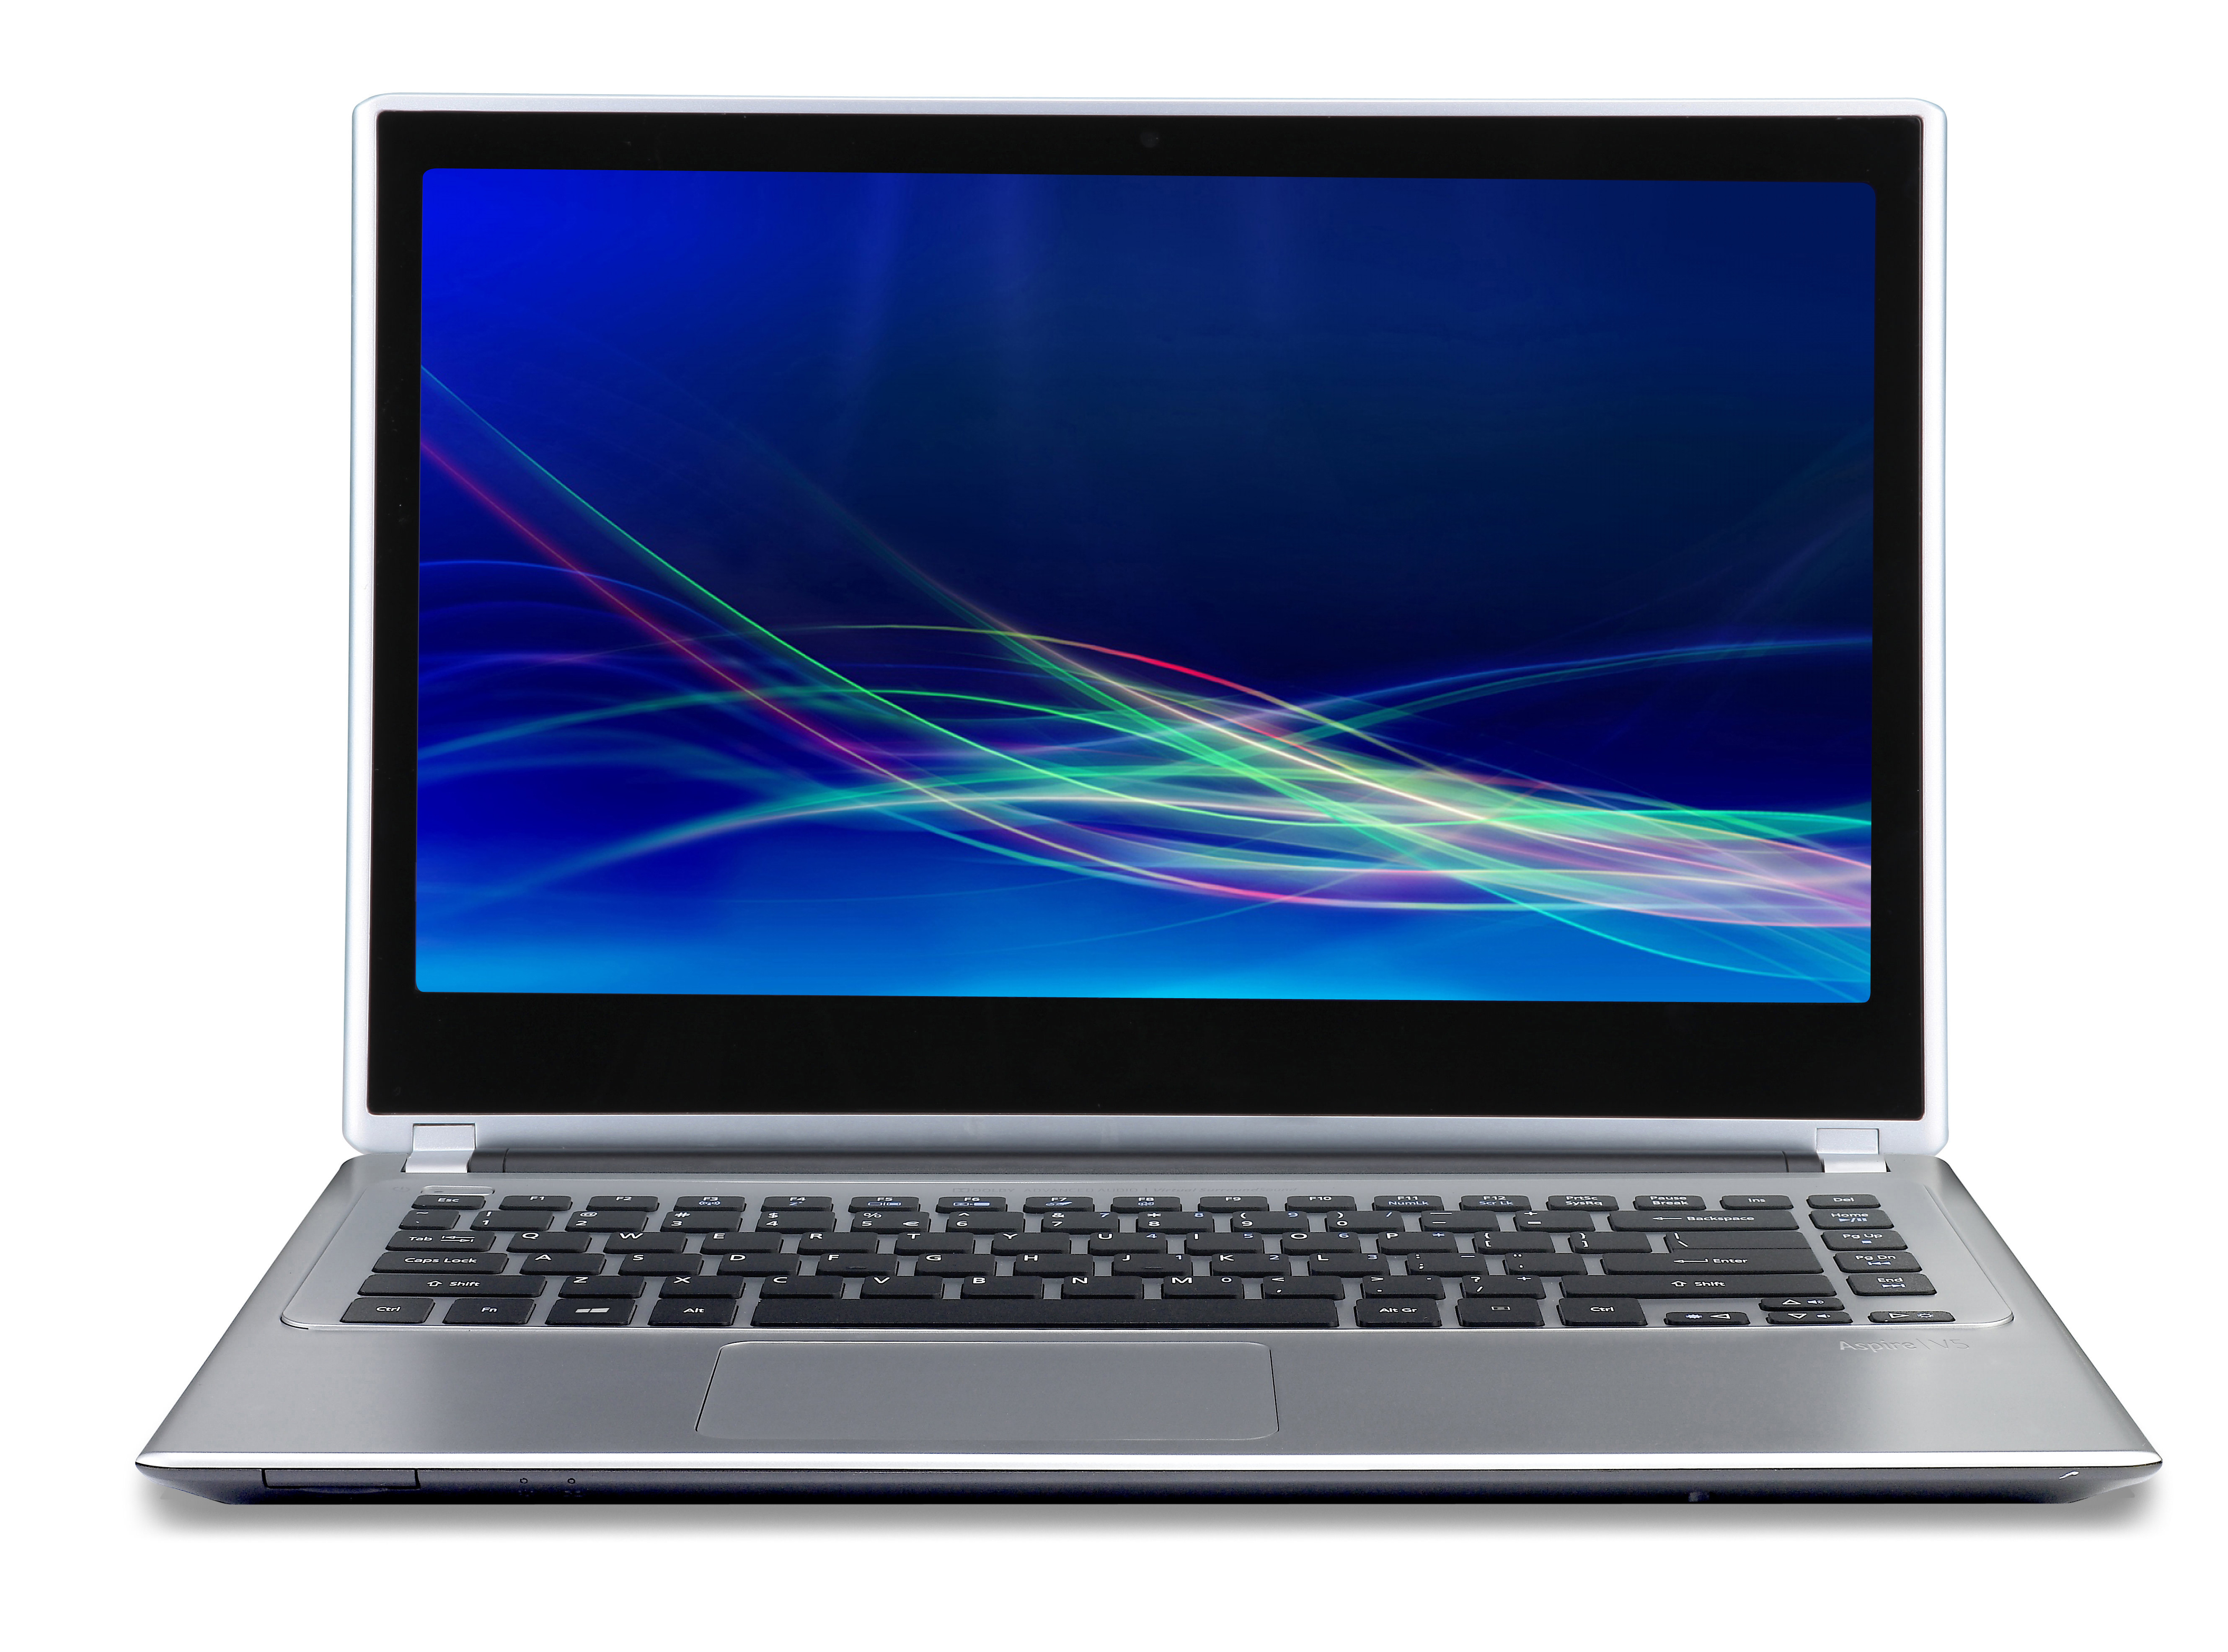
\includegraphics[height=3cm]{figs/notebook.jpg}\hspace{1cm}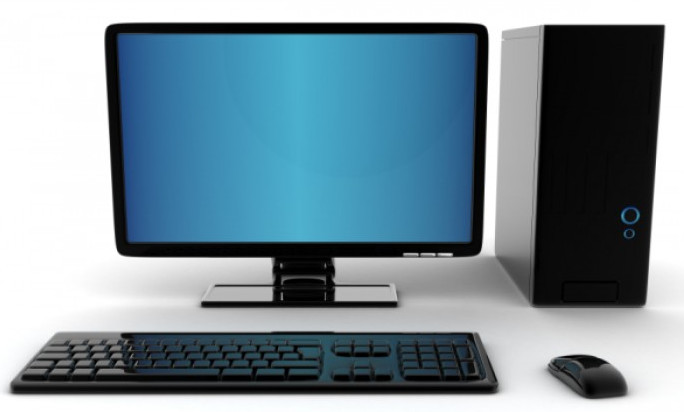
\includegraphics[height=3cm]{figs/desktop.jpg}
\end{center}
\caption{Sistema Inform'atico: Sistema de procesamiento de la informaci'on basado en computadores}
\end{figure}
\end{frame}

\begin{frame}[fragile]\frametitle{Computador}
\begin{itemize}
\item M'aquina capaz de aceptar datos a trav'es de un medio de entrada, procesarlos autom'aticamente bajo el control de un programa previamente almacenado, y proporcionar la informaci'on resultante a trav'es de un medio de salida
\end{itemize}
\end{frame}

\begin{frame}[fragile]\frametitle{Inform'atica}
La Inform'atica se ocupa de la informaci'on como materia esencial de estudio; con esta informaci'on es necesario:
\begin{itemize}
\item \textbf{Representarla} en forma eficiente y automatizable.
\item \textbf{Retransmitirla} sin errores ni pérdidas.
\item \textbf{Almacenarla} para poderla acceder y recuperar tantas veces como sea preciso.
\item \textbf{Procesarla} para obtener nuevas informaciones más elaboradas y más útiles a nuestros propósitos.
\end{itemize}
\end{frame}

\begin{frame}[fragile]\frametitle{Sistema Informático}
\begin{itemize}
\item \textbf{Hardware}: El equipo físico que compone el sistema se conoce con la palabra inglesa \textbf{hardware}, que en castellano se puede traducir como ``soporte físico". Es el conjunto de dispositivos electrónicos y electromecánicos, circuitos, cables, etc., que componen el computador.
\begin{center}
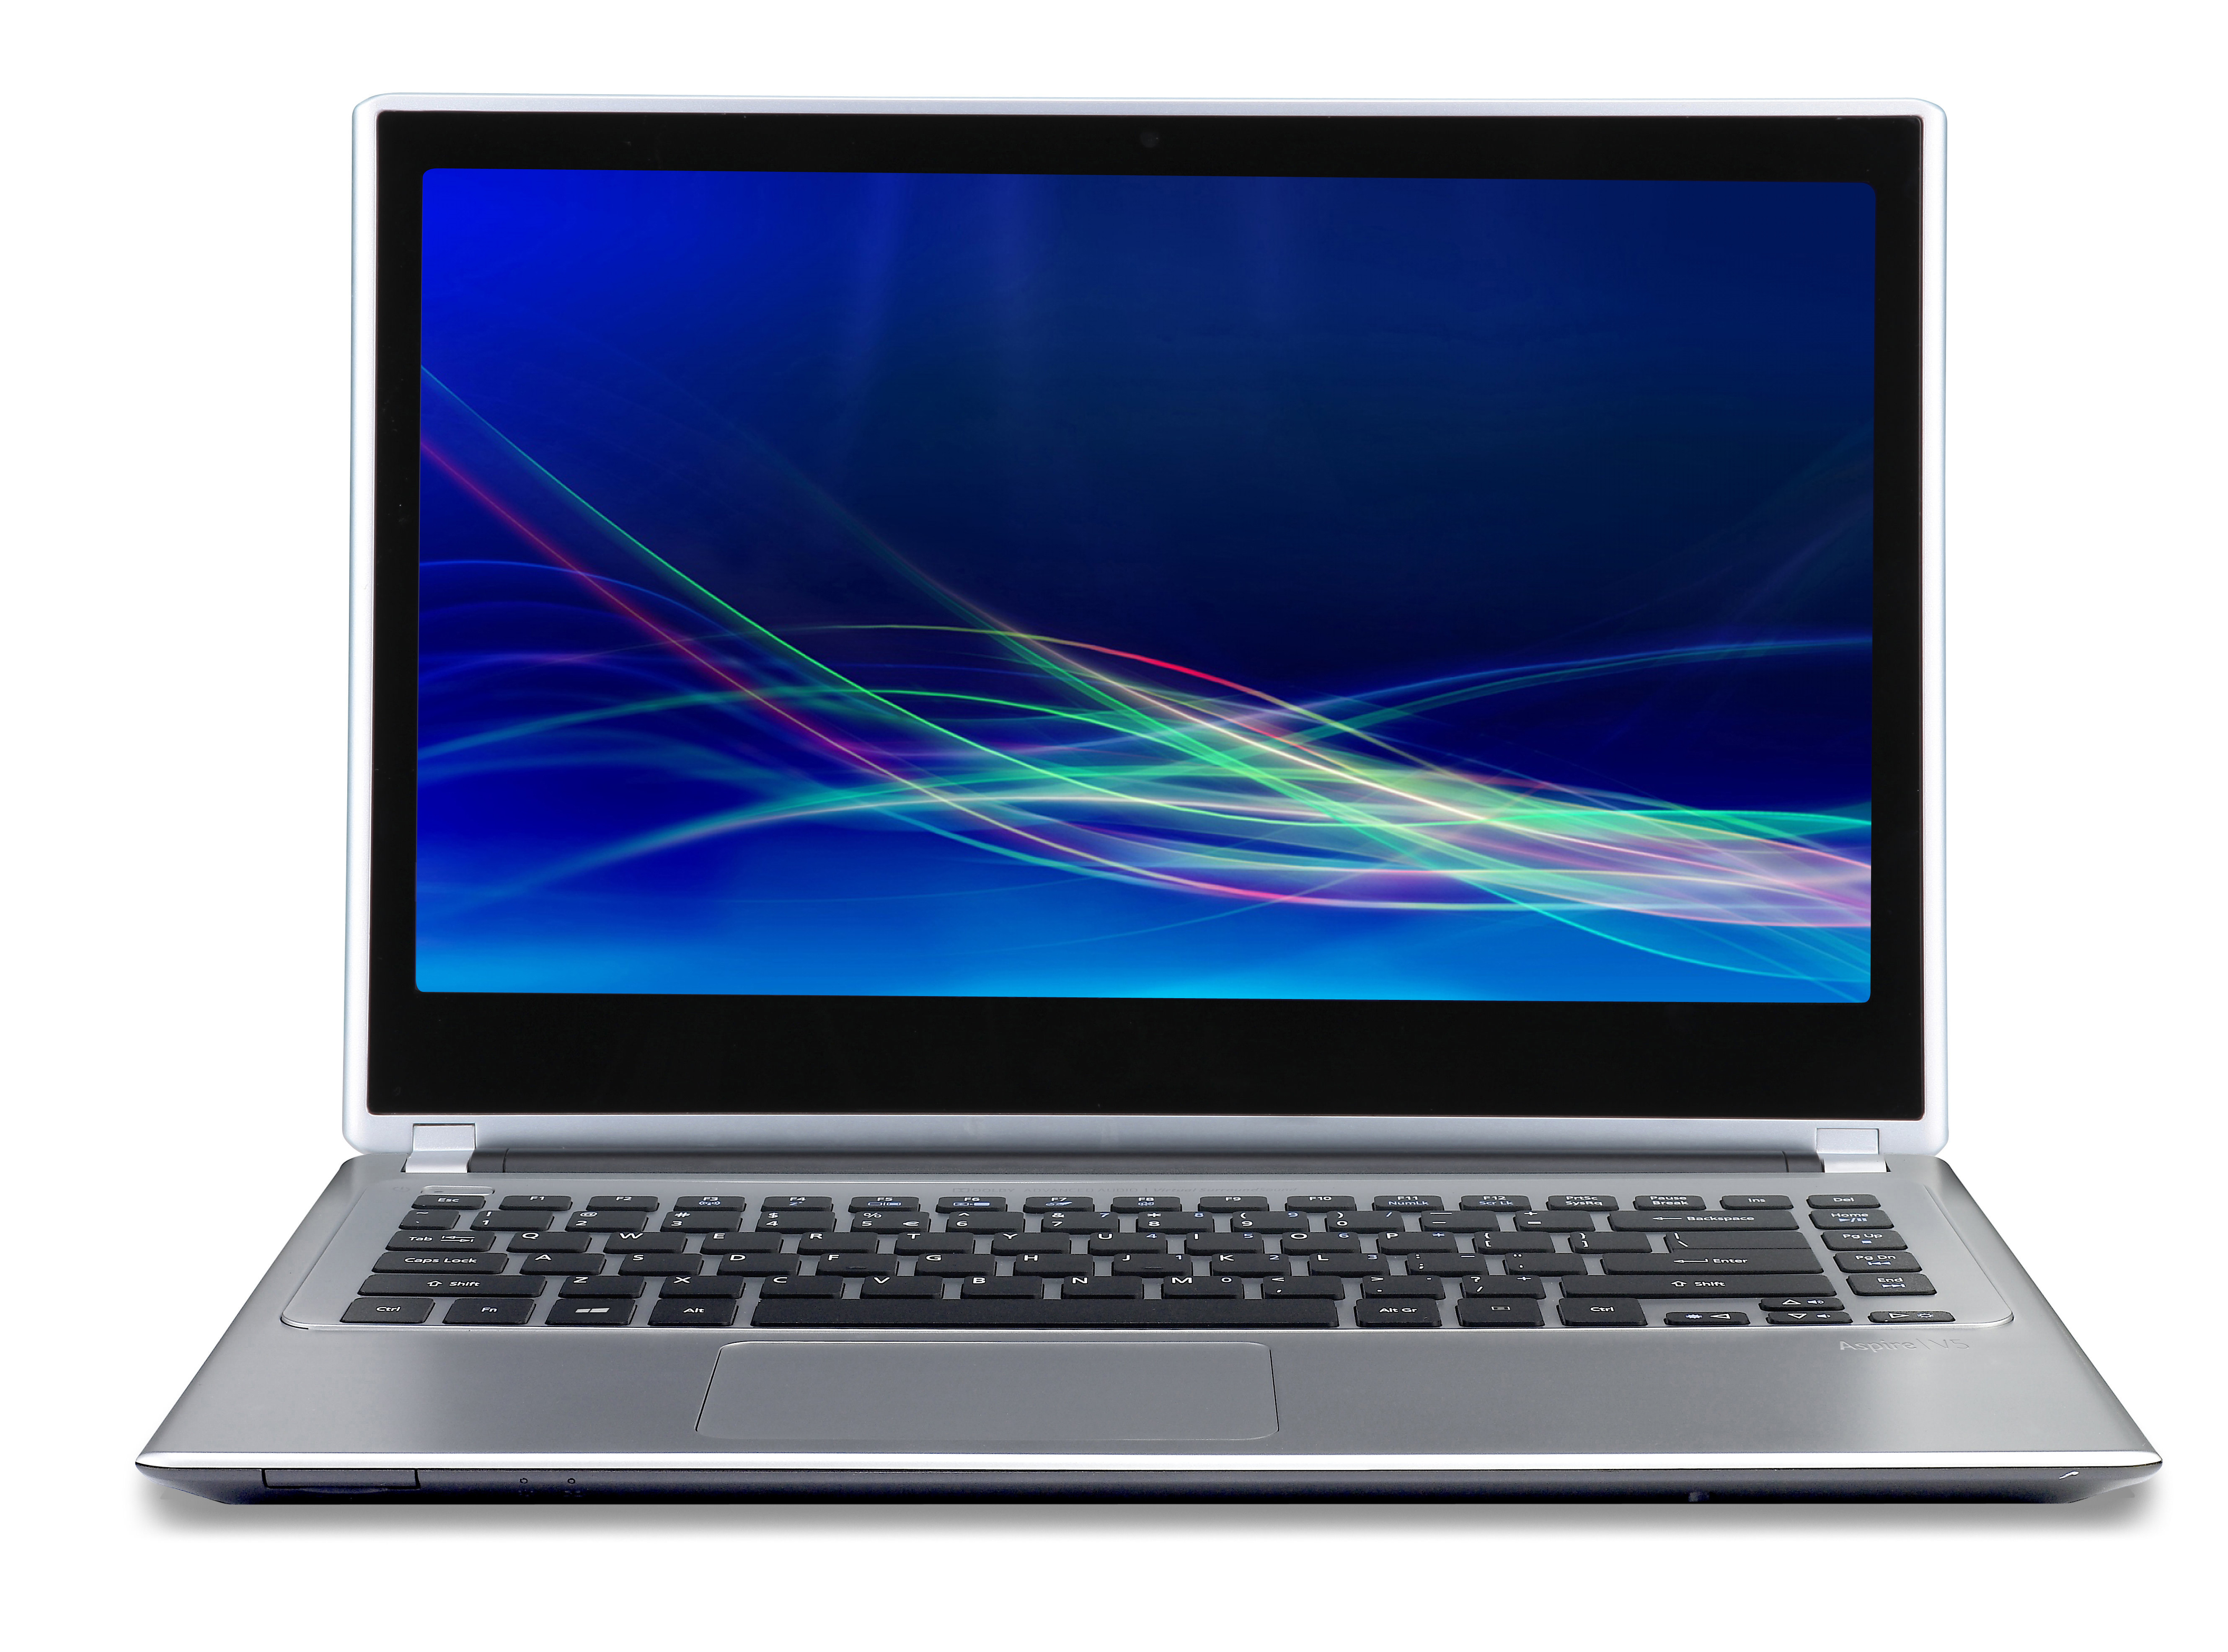
\includegraphics[height=3cm]{figs/notebook.jpg}
\end{center}
\end{itemize}
\end{frame}

\begin{frame}[fragile]\frametitle{Software}
\begin{center}

\includegraphics[height=2cm]{figs/Windows-10.png}\hfill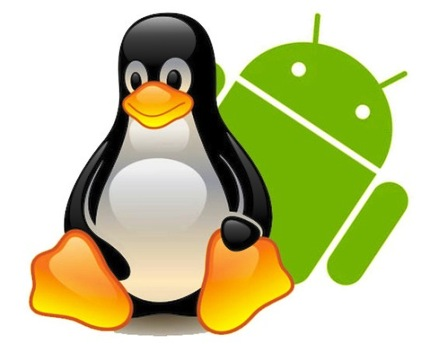
\includegraphics[height=2cm]{figs/linux-android.jpg}\hfill
\includegraphics[height=2cm]{figs/MacOS.jpg}
\end{center}
\begin{itemize}
\item \textbf{Software}: Software: Para que el sistema trabaje, necesita que le suministren una serie de órdenes que indiquen qué es lo que queremos que haga. Estas órdenes se le suministran por medio de \textbf{programas}. El software o ``soporte lógico"\, está compuesto por todos aquellos programas necesarios para que el computador trabaje. El software dirige de forma adecuada a los elementos físicos o hardware.
\end{itemize}
\end{frame}

\section{Medidas de Información}
\begin{frame}[fragile]\frametitle{Medidas de Información}
\begin{itemize}
\item \textbf{El bit (b)} (= Binary Digit): Un elemento con dos posibles estados en el que distinguimos dos valores claramente diferenciados, es una variable binaria, (0 ó 1).
\item Podemos codificar cualquier alfabeto en formato binario, es decir, mediante bits. Cuantos más símbolos contenga el alfabeto más número de bits nos harán falta para codificarlo. Hoy en día es habitual codificar tanto la información visual como la auditiva de alta fidelidad en binario.
\end{itemize}
\end{frame}


\begin{frame}[fragile]\frametitle{Ventajas del Sistema Binario}
\begin{itemize}
	\item Toda la circuitería lógica necesaria para procesar la información en binario (decodificadores, etc) es relativamente sencilla de diseñar y está sumamente estudiada.

\item Existen multitud de dispositivos bi-estables que se pueden emplear para almacenar información codificada en binario:
\begin{itemize}
	\item \textbf{Corriente eléctrica (voltaje)}: distinguir entre 10 o más niveles de voltaje es delicado y caro; distinguir entre pasa/no pasa corriente es muy económico y concede un amplio margen de tolerancia.
	\item \textbf{Intensidad de luz}: luz apagada/luz encendida.
	\item \textbf{Perforación en papel o cartulina}.
	\item \textbf{Sentido de magnetización}: distinguir entre distintos valores de campo magnético es complicado; distinguir entre magnetización Norte--Sur y su contraria Sur--Norte es mucho más fácil y fiable.
\end{itemize}
\end{itemize}
\end{frame}


\begin{frame}[fragile]\frametitle{Medidas de Información}
\begin{itemize}
\item \textbf{El byte (B)}: El byte (típicamente) es el conjunto de 8 bits. Así, en lugar de decir que un mensaje tiene 32 bits, podemos decir que tiene 4 bytes:
$$
1 \text{B} = 8 \text{b}.
$$
Un byte puede por lo tanto adoptar $2^8=256$ estados (valores) distintos. 
\end{itemize}
\end{frame}


\begin{frame}[fragile]\frametitle{Medidas de Información: Múltiplos (k, M, G,...)}
A partir de la propuesta en de la \href{https://es.wikipedia.org/wiki/Comisi%C3%B3n_Electrot%C3%A9cnica_Internacional}{Comisi\'on Electrot\'ecnica Internacional} (IEC) en 1998:
\begin{itemize}
	\item \textbf{k} es la abreviatura de \textbf{kilo}, y representa un factor de multiplicación de mil, es decir $10^3$. Así que 1 kbit = 1000 bits y 1 kbyte = 1000 bytes = 8000 bits. 
	
	\item La \textbf{M} es la abreviatura de \textbf{Mega} y representa el factor de multiplicación de un mill\'on, $10^{6}= $1.000.000.
	
	\item La \textbf{G} es abreviatura de \textbf{Giga} y representa el factor de multiplicación de mil millones, $10^{9} = $1.000.000.000.
\end{itemize}
\end{frame}


\begin{frame}[fragile]\frametitle{Medidas de Información: Múltiplos (k, M, G,...)}

\begin{block}{}
\textbf{Cuidado!:} Estas definiciones a'un no son 100\% adoptadas, ya que anteriormente se prefer'ia usar una base binaria, de modo que la definici\'on previa a 1998 era: 1kB = $2^{10}$ B $=1024$ B, 1MB $=2^{20}$B = 1.048.576 B y 1GB $=2^{30}$B = 1.073.741.824 B, etc. 
\end{block}

\begin{block}{}
Estas viejas definiciones son ahora denotadas como kiB (kibibite), MiB (mebibyte) y  Gib (gibibyte) respectivamente. 
\end{block}
\begin{block}{}
As'i, por ejemplo, 1 MiB = 1.048.576 B = 1,048576 MB.
\end{block}
Ver \url{https://es.wikipedia.org/wiki/Kibibyte} para m'as informaci'on.
\end{frame}


\begin{frame}[fragile]\frametitle{Caracteres}
\begin{itemize}

\item \textbf{El Carácter}: Es la unidad de información \textit{a nivel del alfabeto humano}. Un carácter es, de hecho, \textit{cualquier símbolo del alfabeto usado como alfabeto normal}. Constituye una buena medida de información en términos directamente aplicables a textos expresados en el alfabeto humano.

\item Podemos clasificar los caracteres en:
	\begin{itemize}
		\item \textbf{Alfabéticos}: letras y algún que otro carácter asimilado.
		\item \textbf{Numéricos}: los dígitos numéricos del 0 al 9.
		\item \textbf{Especiales}: todos los restantes (signos de puntuación, signos monetarios, signos de operaciones aritméticas, etc).
	\end{itemize}
	\item Normalmente, en un computador, para representar un carácter se usa 1 byte de informaci'on.
\end{itemize}
\end{frame}


\begin{frame}[fragile]\frametitle{Código de caracteres ASCII}
\begin{block}{}
``\textbf{A}merican \textbf{S}tandard \textbf{C}ode for \textbf{I}nformation \textbf{I}nterchange" (= Código Estándar Estadounidense para el Intercambio de Información, 1963)
\end{block}
\begin{center}
	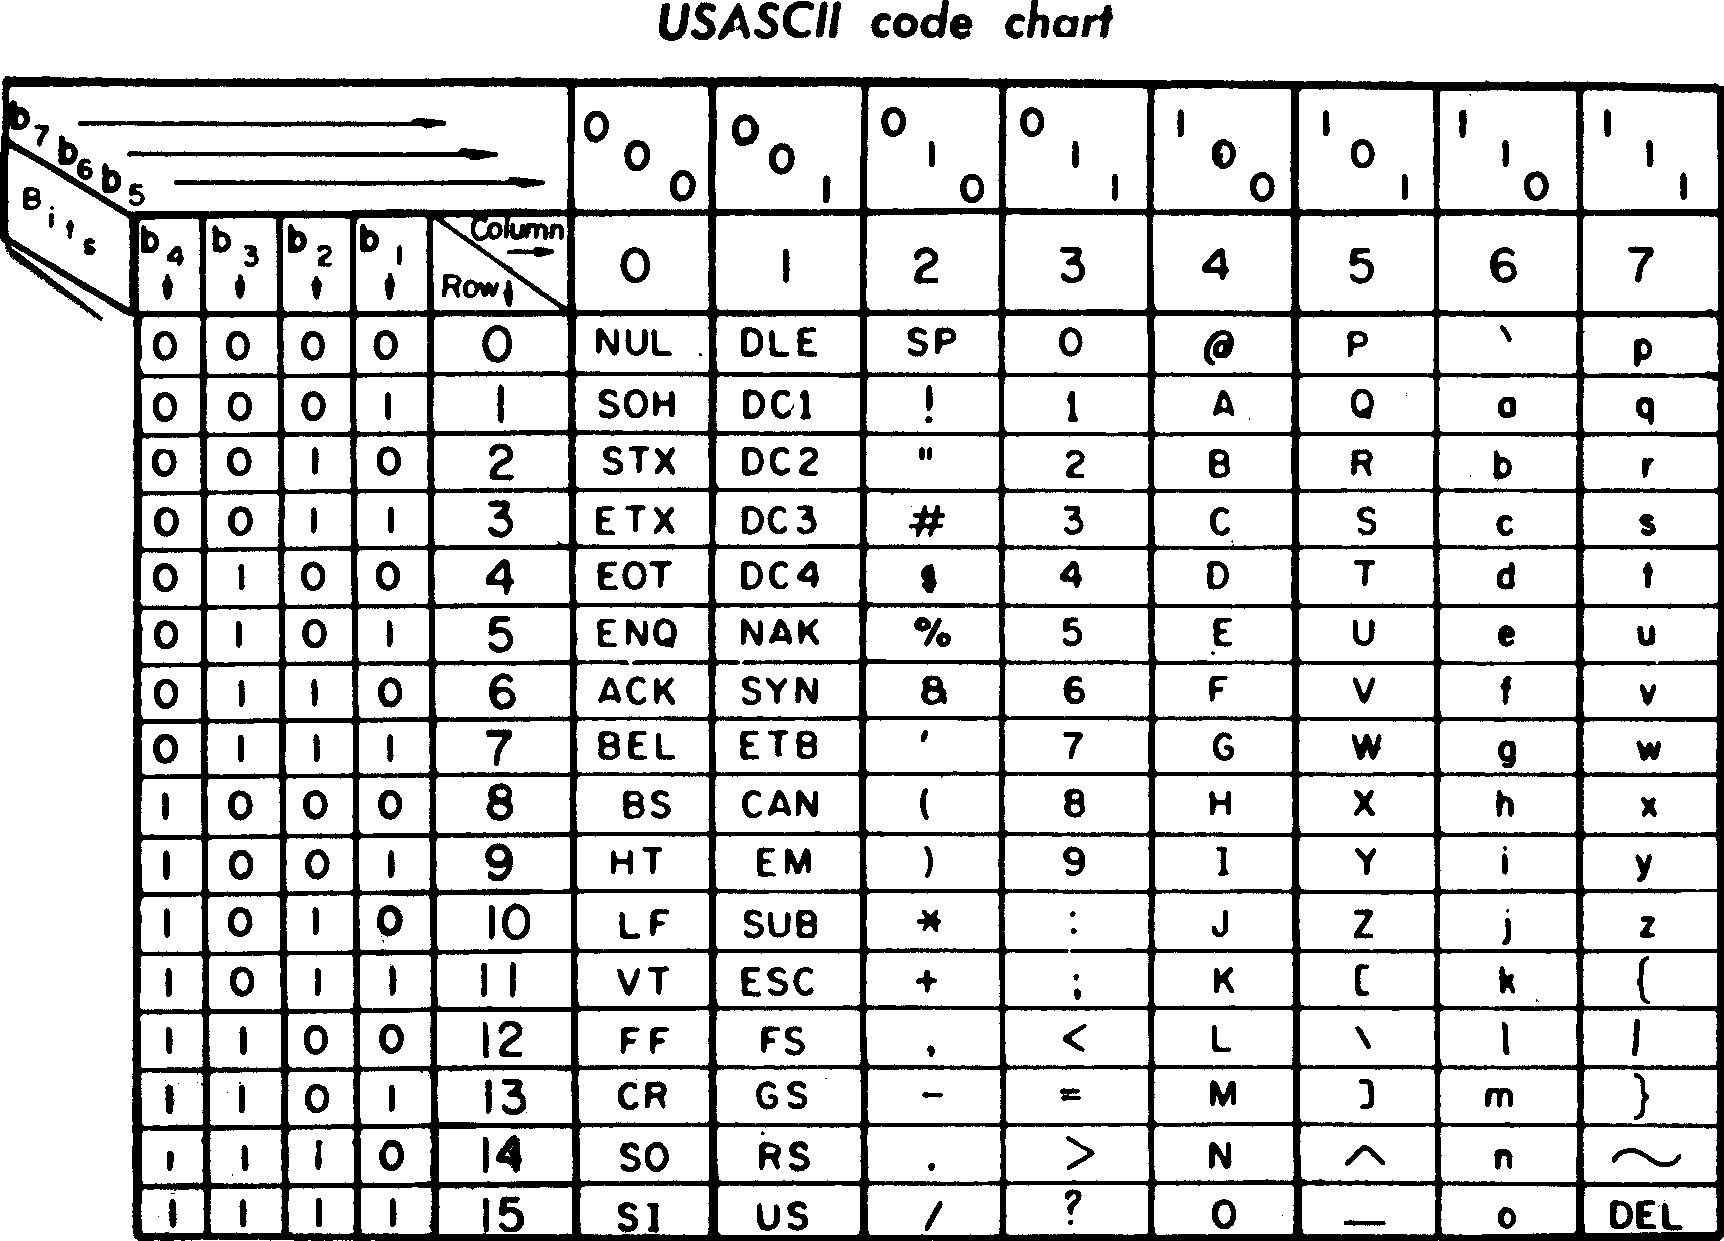
\includegraphics[width=5.5cm]{figs/USASCII_code_chart.png}
\end{center}
 P.ej. ``G" $\rightarrow$ [1000111] $\rightarrow$ 71, \qquad  ``$<$"$ \rightarrow$ [0111100] $\rightarrow$ 60
\end{frame}


\begin{frame}[fragile]\frametitle{Código de caracteres ASCII}
\begin{itemize}
\item Los (95) caracteres imprimibles m'as usados en inform'atica:
\begin{verbatim}
  ! " # $ % & ' ( ) * + , - . / 0 1 2 3 4 5 6 7 8 9 
  : ; < = > ? @ A B C D E F G H I J K L M N O P Q R 
  S T U V W X Y Z [ \ ] ^ _ ` a b c d e f g h i j k 
  l m n o p q r s t u v w x y z { | } ~ 
\end{verbatim}
\item ASCII ordena estos caracteres asoci'andoles un n'umero entre el 32 y el 126. 
\item Otros 32 caracteres no imprimibles, asociados a n'umeros 0 al 31. Representan acciones sobre el texto o el computador. P. ej, activar may'usculas (14) o el pulsar la tecla Suprimir (127). 
\item Listado completo, $32+95 = 127$ caracteres en \href{https://es.wikipedia.org/wiki/ASCII}{Wikipedia}.

\item ASCII original no incorpora 'a'e'i'o'u, ni  \~n. Se crearon extensiones de 8 bits del c'odigo ASCII que incorporan estos y otros caracteres, p.ej. c'odigo \href{https://es.wikipedia.org/wiki/ISO/IEC_8859-1}{ISO 8859-1}.
\end{itemize}
\end{frame}

\begin{frame}[fragile]\frametitle{Unicode/UTF-8}
\begin{itemize}
\item Otro est'andar de codificaci'on de caracteres crecientemente popular es \href{https://es.wikipedia.org/wiki/Unicode}{Unicode}. 
\item Dise\~nado para dar soporte a m'ultiples lenguajes, incluyendo caracteres árabes, japoneses, chinos, griegos, y tambi'en s'imbolos matem'aticos, t'ecnicos, musicales y de otros tipos, incluidos emoticones! 
\item Hoy Unicode posee (versi'on 5.1) 100.713 caracteres, ver p'agina oficial del \href{http://www.unicode.org/charts/}{Consorcio Unicode}, encargado de mantener y actualizar este est'andar. 
\item Una de las implementaciones m'as populares de Unicode es la codificaci'on \href{https://es.wikipedia.org/wiki/UTF-8}{UTF-8} (``8-bit Unicode Transformation Format'', es decir ``Formato de transformaci'on Unicode de 8-bits"). La codificaci'on UTF-8 es la m'as popular en la web.
\end{itemize}
\end{frame}


\section{Sistema Binario}
%\begin{frame}[fragile]\frametitle{Ventajas del Sistema Binario}
%\begin{itemize}
%	\item Toda la circuitería lógica necesaria para procesar la información en binario (decodificadores, etc) es relativamente sencilla de diseñar y está sumamente estudiada.
%\end{itemize}
%\end{frame}

%\begin{frame}[fragile]\frametitle{Ventajas del Sistema Binario}
%\begin{itemize}
%	\item La aritmética en base 2 es la más fácil de implementar. Las reglas de suma, resta, multiplicación y división son las más breves y simples a la hora de construir un circuito lógico que las cumpla. Al disponer de solo dos símbolos (0 y 1), las tablas son muy simples:
%\end{itemize}
%	\begin{center}
%	\begin{tabular}{cccc}
%		 	&  	& $+$ 	& $\times$ \\ \hline
%		0 	& 0	& 0 	& 0 \\
%		0 	& 1	& 1 	& 0 \\
%		1 	& 0	& 1 	& 0 \\
%		1 	& 1	& 10 	& 1 \\
%	\end{tabular}
%	\end{center}
%\end{frame}SO

\section{Licencias de Software}
\begin{frame}[fragile]\frametitle{Licencias de Software}
Una licencia es un \textit{contrato} que estipula los derechos y deberes del creador o distribuidor del software y el usuario (EULA). T'ipicamente, la licencia estipula bajo qu' e condiciones el usuario puede hacer uso del software, si es posible distribuir copias, o hacer modificaciones a 'este.
\begin{itemize}
\item Software propietario. 
\item Shareware
\item Freeware
\item Software Libre
\end{itemize}
\end{frame}

\end{document}